\documentclass[11pt,a4paper]{article}
\usepackage[utf8]{inputenc}
\usepackage[T1]{fontenc}
\usepackage{tgpagella}
\usepackage[spanish]{babel}
\usepackage{geometry}
\usepackage{booktabs}
\usepackage{xcolor}
\usepackage{titlesec}
\usepackage{fancyhdr}
\usepackage[parfill]{parskip}
\usepackage[expansion=false]{microtype}
\usepackage{hyperref}
\usepackage{setspace}
\usepackage{needspace}
\usepackage{graphicx}
\widowpenalty=10000
\clubpenalty=10000
\displaywidowpenalty=10000

\geometry{top=3.0cm,bottom=3.0cm,left=3.5cm,right=3.5cm}
\setlength{\parskip}{0.65em}
\setlength{\parindent}{0em}

\definecolor{azulai}{RGB}{30,80,140}
\definecolor{doradoai}{RGB}{140,90,0}
\definecolor{grisai}{RGB}{70,70,70}

\titleformat{\section}{\Large\bfseries\color{azulai}}{}{0em}{}[{\color{azulai}\titlerule[0.5pt]}]
\titlespacing*{\section}{0pt}{1.8em}{0.8em}
\titleformat{\subsection}{\large\bfseries\color{doradoai}}{}{0em}{}
\titlespacing*{\subsection}{0pt}{1.4em}{0.5em}
\titleformat{\subsubsection}{\normalsize\bfseries\color{grisai}}{}{0em}{}
\titlespacing*{\subsubsection}{0pt}{1.0em}{0.3em}

\pagestyle{fancy}\fancyhf{}
\rhead{\textcolor{grisai}{\small Nieves Arrarás — Arquitectura Interna}}
\lhead{\textcolor{grisai}{\small Sol · Ascendente · Nodos}}
\cfoot{\textcolor{grisai}{\small\thepage}}
\renewcommand{\headrulewidth}{0.3pt}

\hypersetup{colorlinks=true,linkcolor=azulai,urlcolor=azulai}
\setstretch{1.45}
\tolerance=1500
\emergencystretch=4em

\begin{document}

% ── Portada ──────────────────────────────────────────────────────────────────
\begin{titlepage}
  \centering
  \vspace*{1.5cm}
  {\Huge\bfseries\color{azulai} Sol · Ascendente · Nodos}\\[0.5cm]
  {\large\color{grisai} Arquitectura Interna}\\[0.3cm]
  {\small\itshape\color{grisai} Dirección vital, punto de entrada y eje de desarrollo}\\[2cm]
  {\huge\color{doradoai} Nieves Arrarás}\\[1.5cm]
  {\Large 01/12/1948 \quad 01:20}\\[0.3cm]
  {\Large Pamplona, España}\\[0.3cm]
  {\normalsize Lat: 42.8157° \quad Lon: -1.6522° \quad UTC+01:00}\\[0.3cm]
  {\normalsize Ascendente: Virgo 16°53' \quad
    MC: Géminis 14°27'}\\[2cm]
  \begin{tabular}{lll}
    \textbf{Sol:} & Sagitario & Casa 3 \\
    \textbf{Ascendente:} & Virgo & Punto de entrada principal: Mercurio \\
    \textbf{Nodo Norte:} & Tauro & Casa 8 \\
    \textbf{Nodo Sur:}   & Escorpio & Casa 2 \\
  \end{tabular}\\[2cm]
  \vfill
  {\small Generado el 14/05/2026}
\end{titlepage}

\tableofcontents
\newpage

% ── Datos de referencia ───────────────────────────────────────────────────────
\section{Datos de referencia}

\begin{center}
\begin{tabular}{llll}
  \toprule
  \textbf{Punto} & \textbf{Signo} & \textbf{Casa} & \textbf{Posición} \\
  \midrule
  Sol           & Sagitario & 3 & 8°44' \\
  Ascendente    & Virgo & --- & 16°53' \\
  Medio Cielo   & Géminis & --- & 14°27' \\
  Nodo Norte    & Tauro & 8 & 4°38' \\
  Nodo Sur      & Escorpio & 2 & 4°38' \\
  \bottomrule
\end{tabular}
\end{center}

\vspace{0.5cm}
\textbf{Regente del Ascendente (Virgo):} 
Mercurio —
Sagitario, 
Casa 3

\vspace{0.5cm}
\textbf{Aspectos entre Sol, Ascendente y Nodos:}

\vspace{0.3cm}
\textit{No aparecen aspectos directos entre Sol, Ascendente y Nodos dentro de los orbes definidos. Esto no significa ausencia de relación entre estos puntos, sino que la lectura se apoya principalmente en sus signos, casas, elementos e integración general.}

\vspace{0.7cm}

\begin{center}
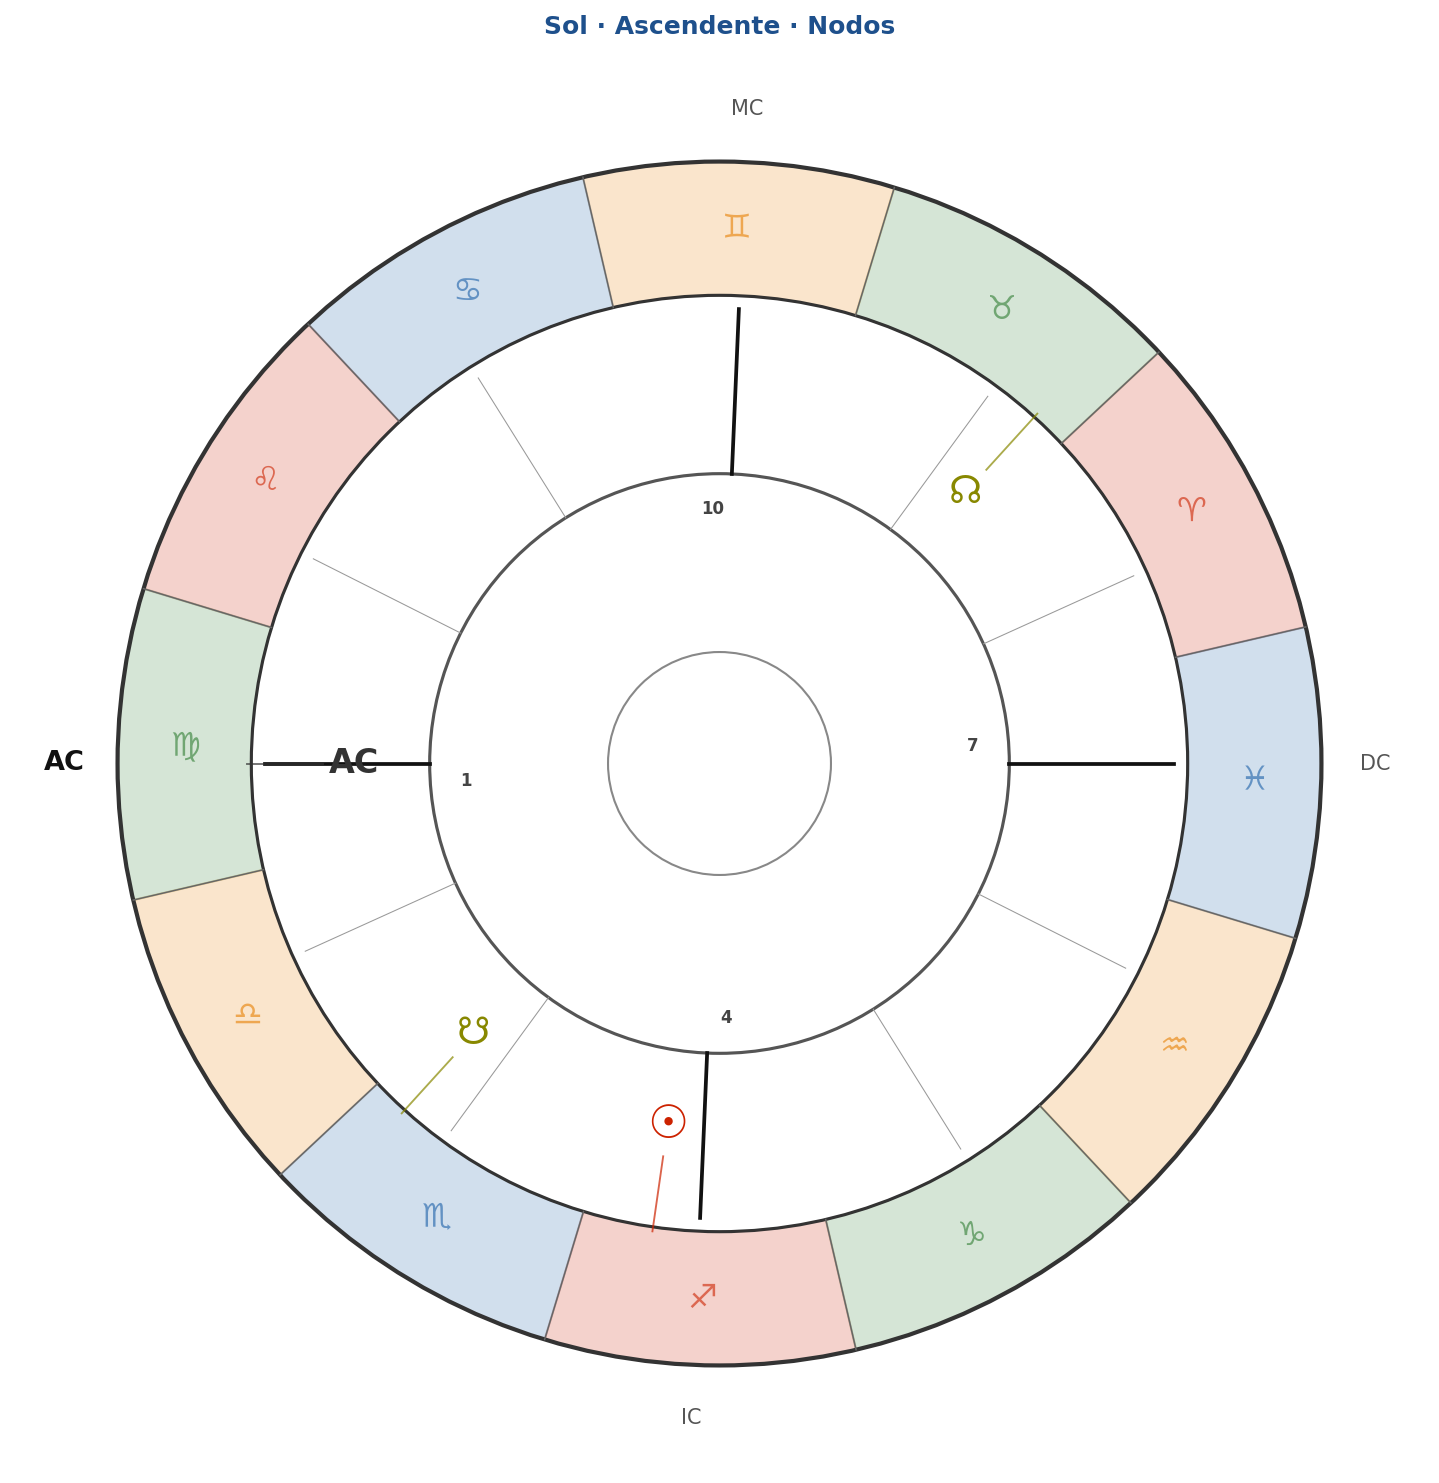
\includegraphics[width=0.72\textwidth]{Nieves_Arrarás_Sol_ASC_Nodos_rueda.png}
\end{center}

\needspace{3\baselineskip}
\subsection*{Grados sensibles}



\newpage

% ── Interpretación ────────────────────────────────────────────────────────────
\section{Interpretación — Arquitectura Interna}

\begin{center}
{\small\itshape
No se trata de definir quién eres. Se trata de observar cómo se organiza tu dirección,
cómo atraviesas la vida y qué tensión influye en tu forma de avanzar.
}
\end{center}

\vspace{0.5cm}

% ── 1. Dirección general ──────────────────────────────────────────────────────
\needspace{3\baselineskip}
\subsection{1. Dirección general}

El Sol está en Sagitario, Casa 3. El Ascendente está en Virgo. El Nodo Norte está en Tauro, Casa 8, y el Nodo Sur en Escorpio, Casa 2.

El Sol en Sagitario y el Ascendente en Virgo pertenecen a elementos con lógicas diferentes. Esto puede hacer que vivas las cosas de una forma, mientras otra parte de ti necesita orientarse desde un ritmo completamente diferente.

El Sol en Sagitario, Casa 3, no tiene un aspecto directo con los Nodos. La tensión entre el Nodo Norte en Tauro, Casa 8, y el Nodo Sur en Escorpio, Casa 2, se expresa de una forma más independiente respecto a la dirección solar.

\vspace{0.6cm}

% ── 2. Sol ────────────────────────────────────────────────────────────────────
\needspace{3\baselineskip}
\subsection{2. El Sol — Dirección principal}

\needspace{3\baselineskip}
\subsubsection*{Sol en Sagitario · Casa 3}

Tu dirección se activa cuando sientes que hay un horizonte hacia el que crecer. Necesitas sentido, expansión y la sensación de que tu vida se mueve hacia algo más amplio.

La rutina por sí sola rara vez te sostiene. Necesitas comprender por qué haces lo que haces y sentir que hay una dirección con significado detrás.

Puedes entusiasmarte con muchas posibilidades al mismo tiempo y perder fuerza intentando abarcar demasiado. También te afecta vivir en contextos demasiado cerrados, repetitivos o limitados. Cuando pierdes sentido, aparece desorientación antes que tristeza.

Tu dirección se activa a través del intercambio con el entorno cercano. Necesitas hablar, aprender, pensar, conectar ideas o moverte entre distintas conversaciones y estímulos.

Cuando no puedes expresarte o sientes que tu mente se queda encerrada demasiado tiempo en lo mismo, aparece inquietud rápidamente.

Sueles encontrar claridad mientras hablas, escribes, preguntas o compartes lo que piensas. La dirección aparece en movimiento, no en aislamiento prolongado.


\vspace{0.6cm}

% ── 3. Ascendente ─────────────────────────────────────────────────────────────
\needspace{3\baselineskip}
\subsection{3. El Ascendente — Forma de relacionarte con la vida}

\needspace{3\baselineskip}
\subsubsection*{Virgo · Regente: Mercurio}

Sueles necesitar comprender, ordenar o ajustar lo que estás viviendo para poder procesarlo bien.Muchas veces observas rápidamente los detalles, lo que falta o lo que podría hacerse mejor.

Cuando el entorno es muy caótico o no hay tiempo para procesar lo que ocurre, puede aparecer ansiedad, irritación o sensación de tener algo pendiente todo el tiempo.

Te ayuda sentir cierta claridad, coherencia y espacio para entender bien las cosas antes de seguir acumulando experiencia.

El regente del Ascendente es Mercurio, situado en Sagitario, Casa 3. Mercurio pertenece a un elemento con una lógica diferente a la del Ascendente. Esto puede hacer que vivas las cosas de una forma, mientras otra parte de ti necesita orientarse desde un ritmo completamente diferente.. La Casa 3 muestra un territorio importante desde el que organizas tu forma de entrar en la vida.

\vspace{0.6cm}

% ── 4. Nodos ──────────────────────────────────────────────────────────────────
\needspace{3\baselineskip}
\subsection{4. Nodo Norte y Nodo Sur — Dirección de crecimiento}

\needspace{3\baselineskip}
\subsubsection*{Nodo Norte en Tauro · Casa 8 \\
Nodo Sur en Escorpio · Casa 2}

Tu dirección pide construir algo estable, sencillo y sostenible en el tiempo. Desarrollar recursos propios, aprender a ir despacio y confiar más en lo concreto.

Lo conocido suele llevarte hacia la intensidad emocional, las crisis o los procesos de transformación profunda. Hay una tendencia a sentir que solo lo intenso es verdadero o importante.

El reto está en descubrir que la calma, la estabilidad y lo cotidiano también pueden tener profundidad. Crecer hacia este Nodo Norte implica dejar de necesitar constantemente situaciones límite para sentir que algo es real.

Tu dirección pide entrar más profundamente en los procesos de cambio y transformación. Aprender a soltar lo que ya terminó y atravesar etapas donde no todo está bajo control.

El crecimiento aparece cuando puedes dejar atrás viejas seguridades y permitir que algunas partes de tu vida cambien de verdad.

El reto suele estar en no quedarte únicamente en lo estable o conocido por miedo a perder estructura.

Sueles vivir lo que te pasa con mucha intensidad y profundidad, como si las cosas necesitaran transformarte de alguna manera.

Hay facilidad para entrar en lo complejo, sostener crisis o percibir lo que otras personas no ven, pero también tendencia a vivir en tensión constante.

El problema aparece cuando solo puedes sentir que algo es real si tiene intensidad, conflicto o carga emocional profunda.

Tiendes a buscar seguridad en lo conocido, en lo estable y en aquello que puedes controlar o conservar.

Hay facilidad para construir recursos y sostener continuidad, pero también dificultad para entrar en cambios profundos cuando implican incertidumbre o pérdida de control.

El problema aparece cuando mantener estabilidad se vuelve más importante que reconocer que algo necesita transformarse.

\vspace{0.6cm}

% ── 5. Integración ────────────────────────────────────────────────────────────
\needspace{3\baselineskip}
\subsection{5. Integración — Cómo se relacionan las distintas partes}

El Ascendente en Virgo y el Sol en Sagitario pertenecen a elementos con lógicas diferentes. Esto puede hacer que una parte de ti quiera vivir las cosas de una forma, mientras otra necesita avanzar desde un ritmo completamente diferente.Cuando no hay espacio para traducir esas dos formas internas, puedes sentir que reaccionas por un lado y deseas orientarte por otro. El trabajo está en no forzarte a elegir una sola parte, sino en aprender a darles un lugar más coherente.

El Ascendente en Virgo y el Nodo Norte en Tauro pertenecen al mismo elemento. La forma en la que vives las cosas de manera natural puede ayudarte a avanzar hacia tu dirección de crecimiento, siempre que haya consciencia en ello.El reto está en no repetir automáticamente lo que ya conoces solo porque se parece a lo que también necesitas desarrollar.

\vspace{0.6cm}

% ── 6. Orientación práctica ───────────────────────────────────────────────────
\needspace{3\baselineskip}
\subsection{6. Orientación práctica}

\needspace{3\baselineskip}
\subsubsection*{Desde dónde empezar}
Desde el Ascendente en Virgo: dar un paso concreto, pequeño y verificable. Te ayuda tocar la realidad antes de intentar entenderlo todo mentalmente.

\needspace{3\baselineskip}
\subsubsection*{Qué conviene sostener}
El Sol en Sagitario, Casa 3, necesita una dirección activa: algo que iniciar, decidir o llevar adelante. Si no hay movimiento real, la energía puede convertirse en irritación, urgencia o acción sin rumbo claro.

\needspace{3\baselineskip}
\subsubsection*{Qué conviene observar}
Evita funcionar únicamente desde el Nodo Sur en Escorpio, Casa 2. Ese lugar puede resultarte conocido y eficaz, pero no debería convertirse en la única respuesta disponible. La señal de alerta aparece cuando resuelves siempre desde lo que ya sabes hacer, sin preguntarte si esa respuesta sigue siendo adecuada.

El Nodo Norte en Tauro, Casa 8, pide desarrollar una forma nueva de orientarte, aunque al principio resulte menos automática.

\vspace{1cm}

\begin{center}
{\small\itshape\color{grisai}
La astrología se utiliza aquí como una herramienta de observación y orientación.
No define quién eres ni determina lo que va a ocurrir.
}
\end{center}

\end{document}
